\title{Master Project - Real Time Rendering of skeletal structures - Motivations Goals and Plan}
\author{
        %\large
        \textsc{Olivier Rouiller - s090842}
        \mbox{}\\ %
        Department of Informatics and Mathematical Modelling\\
        Technical University of Denemark\\
        \mbox{}\\ %
}
\date{\today}
\documentclass[11pt]{article}
%\documentclass{acmconf}

\usepackage[paper=a4paper,dvips,top=1.5cm,left=1.5cm,right=1.5cm,
    foot=1cm,bottom=1.5cm]{geometry}

\usepackage{times}
%\usepackage{graphicx}
\usepackage[fleqn]{amsmath}
\usepackage{amsfonts}
\usepackage{amssymb}
\usepackage{amsthm}
\usepackage{amsopn}
\usepackage{xspace}
\usepackage{array}
\usepackage{epsfig}
\usepackage{cite}
\usepackage{pdfpages} 
\usepackage{subfig}



\numberwithin{figure}{section}

\newcommand\CC{\Lang{\mbox{C++}}\xspace}
\newcommand\Lang[1]{\textsc{#1}}
\newcommand{\kw}[1]{\texttt{\textbf{#1}}}
\newcommand{\cd}[1]{\texttt{#1}}

\newcommand\Naturals{\ensuremath{\mathbb{N}}\xspace}
\newcommand\Integers{\ensuremath{\mathbb{Z}}\xspace}
\newcommand\Rationals{\ensuremath{\mathbb{Q}}\xspace}
\newcommand\Reals{\ensuremath{\mathbb{R}}\xspace}
\newcommand\Complex{\ensuremath{\mathbb{C}}\xspace}

\newcommand\norm[1]{\ensuremath{\lVert#1\rVert}}
\newcommand\abs[1]{\ensuremath{\lvert#1\rvert}}
\newcommand\ceil[1]{\ensuremath{\lceil#1\rceil}}
\newcommand\floor[1]{\ensuremath{\lfloor#1\rfloor}}
\newcommand\set[1]{\ensuremath{\{#1\}}}
\newcommand\angular[1]{\ensuremath{\langle#1\rangle}}

\newcommand\Norm[1]{\ensuremath{\left\lVert#1\right\rVert}}
\newcommand\Abs[1]{\ensuremath{\left\lvert#1\right\rvert}}
\newcommand\Ceil[1]{\ensuremath{\left\lceil#1\right\rceil}}
\newcommand\Floor[1]{\ensuremath{\left\lfloor#1\right\rfloor}}
\newcommand\Set[1]{\ensuremath{\left\{#1\right\}}}
\newcommand\Angular[1]{\ensuremath{\left\langle#1\right\rangle}}

\newcommand{\LOOM}{\ensuremath{\cal{LOOM}}\xspace}
\newcommand{\PolyTOIL}{\textbf{PolyTOIL}\xspace}

\newtheorem{theorem}{Theorem}[section]
\newtheorem{definition}[theorem]{Definition}
\newtheorem{lemma}[theorem]{Lemma}
\newtheorem{corollary}[theorem]{Corollary}
\newtheorem{fact}[theorem]{Fact}
\newtheorem{example}[theorem]{Example}

\newcommand\Cls[1]{\textsf{#1}}
\newcommand\Fig[1]{Figure~\ref{Figure:#1}}

\usepackage{labels} %
\usepackage{equation}

\newenvironment{excerpt}{\begin{quote}\begin{minipage}\textwidth}{\end{minipage}\end{quote}}

\setcounter{topnumber}{0}
\setcounter{bottomnumber}{0}
\setcounter{totalnumber}{20}
\renewcommand{\textfraction}{0.01}

\begin{document}

\maketitle

\Section[simple]{Introduction}
	
Graphics modelling is usually done at the polygonal level, models are defined by a polygonal meshes, normals, uv maps and textures. On top of this representation, we often create a skeleton for mesh animation. This representation is well suited to the real time rendering pipeline since polygons can be rendered efficiently by the graphics card.

In the other hand, this modelling process is time consuming and alternative ways of modelling are possible. We are indeed interested in modelling with implicit surfaces ans skeletons. Implicit surfaces are iso-level sets of 3d real functions. Implicit surfaces are interesting because they have a very compact representation, because they can be rendered using different techniques and because they can be used to model smooth surfaces easily by performing operations on them.

The most common examples are metaballs , which blend together



\Section[simple]{Skeletal representation of the model - Work done}

We use a simple skeletal data structure similar to an skeleton for animation. Bones are defined by an orientation (quaternion), a length and a position. The orientations and positions are hierarchical but we also store and maintain world space informations.

\begin{figure}[!h!]
  \centering
  \subfloat[Skeleton]{\label{fig:gull}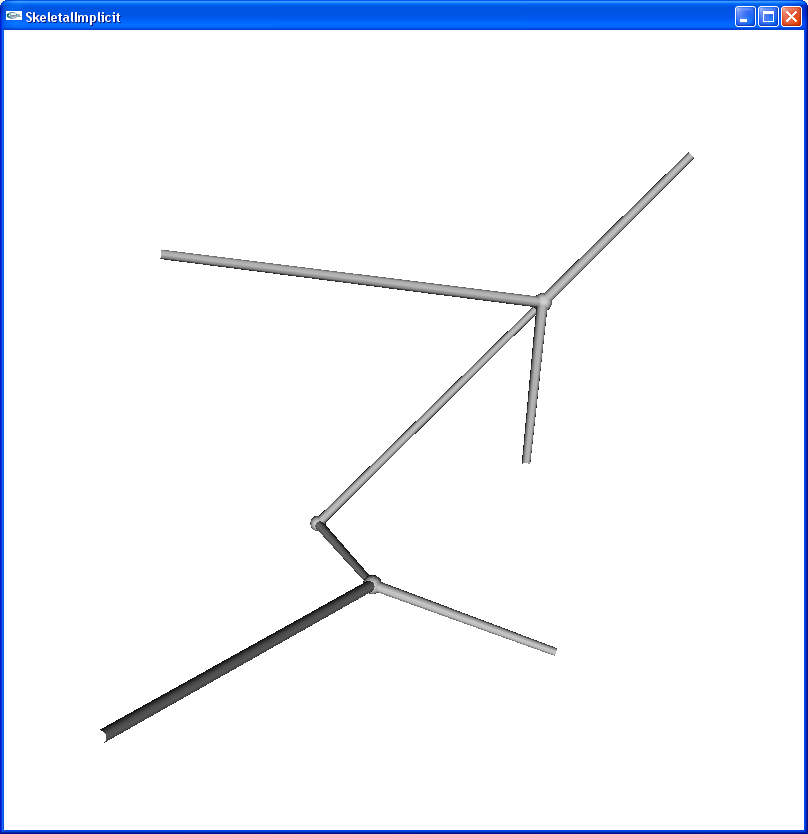
\includegraphics[width=0.4\textwidth]{../pictures/dynamicSkeleton.png}}                
  \subfloat[Primitives representation]{\label{fig:tiger}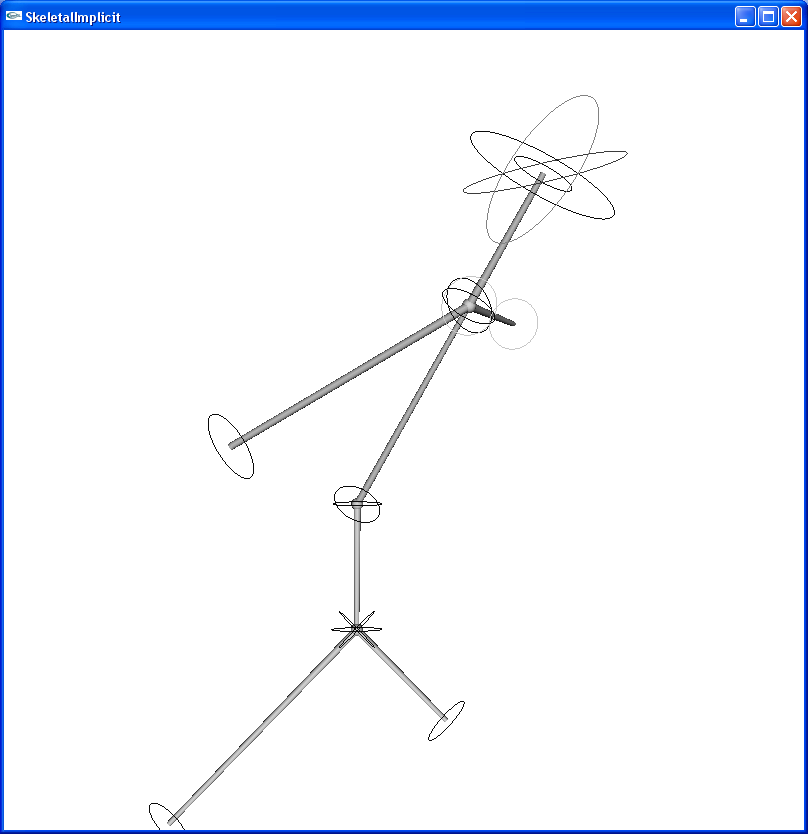
\includegraphics[width=0.4\textwidth]{../pictures/PrimitiveGuysmos.png}}
  \caption{Skeleton and primitives representation}
  \label{fig:animals}
\end{figure}

Each bone has a list of primitives (metatubes and metaballs for now). These primitives have info on the base geometry (segments or points and radius) in local and world space.

I have implemented support for selection of bones and modification, it shouldn't be too hard to implement dynamic creation of bones and edition of the primitives.

\Section[simple]{Raytracing of the structure - Work done}

\subsection{Ray tracing}

Ray tracing is a rendering technique where for each pixel of an image we try to simulate the path of the light from the scene to the pixel.
To do so we throw a ray into the scene, find the intersection of the ray with the geometry of the scene, compute the color of the object at this point and write it to the pixel. To compute the color we can use a simple shading or throw other rays to get a better idea of the light incoming to this point. 

\subsection{Ray tracing of implicit surfaces}

Implicit surfaces can be ray traced because it is easy to find the intersection of the surface with the ray, it boils down to finding the zeros of a function along the ray.

The main issue is to find these zeros efficiently.
The way we did it now is the most naive possible, we go through the ray with a constant step length and stop when the sign of the function value changes.

\subsection{Basics of GPU raytracing of implicit surfaces}

Although ray tracing have been mostly used for offline renderers because of the cost of this technique, with programmable pipelines it is now possible to do ray tracing in real time.
The ray tracing is done in the fragment shader.
To gain efficiency, we need to throw rays only where we know that they are likely to intersect the surface.

To limit the number of rays shot, bounding meshes for the primitives are drawn Figure\ref{bound}.
Info about position and radius of the primitives are sent to the fragment shader in world space.
Rays are shot from the bounding mesh in world space to find the isosurface.
To find the isosurface, all primitives are evaluated which should be avoided. Primitives are sent to the shader as a list of points and radius. Since there is no dynamic allocation of arrays on shaders??
a large enough array is allocated.
The surface is the same as the polygonised surface. But it is a lot faster faster to render it from polygons (2000fps against $<100$).


\begin{figure}[!h!]
  \centering
  \subfloat[Primitives Bounding meshes]{\label{bound}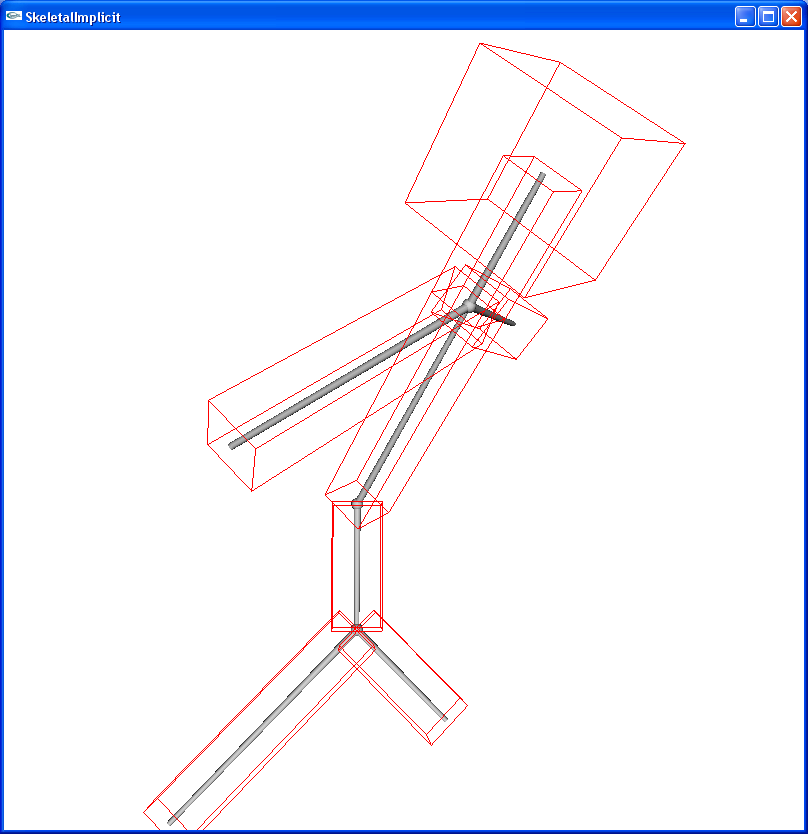
\includegraphics[width=0.3\textwidth]{../pictures/BoundingMeshes.png}}                
  \subfloat[Raytraced isosurface]{\label{fig:tiger}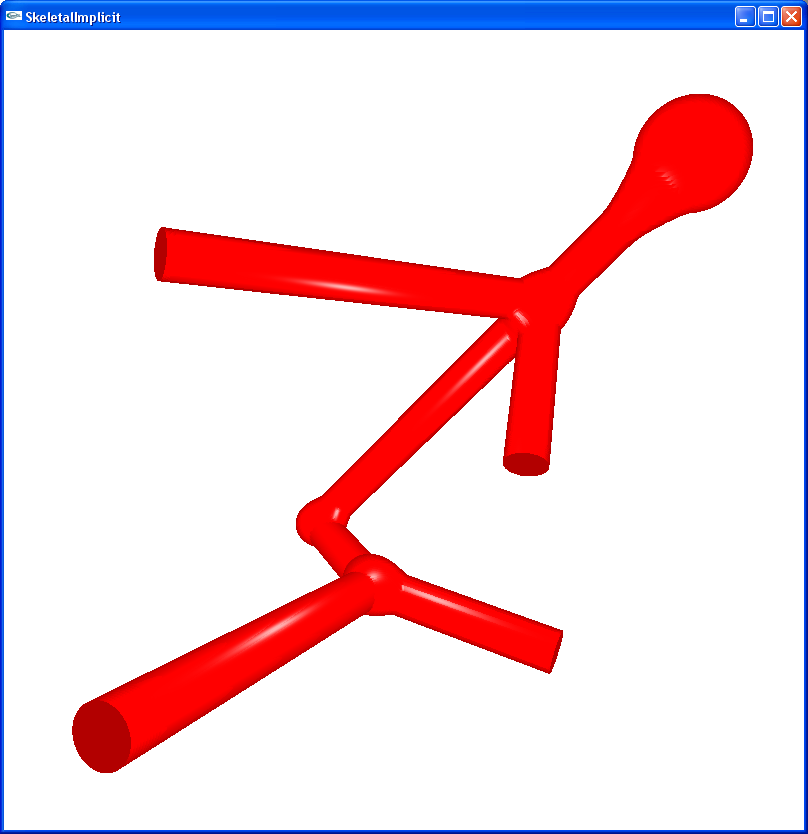
\includegraphics[width=0.3\textwidth]{../pictures/dynamicSkeletonTraced.png}}
    \subfloat[Polygonized surface.]{\label{fig:tiger}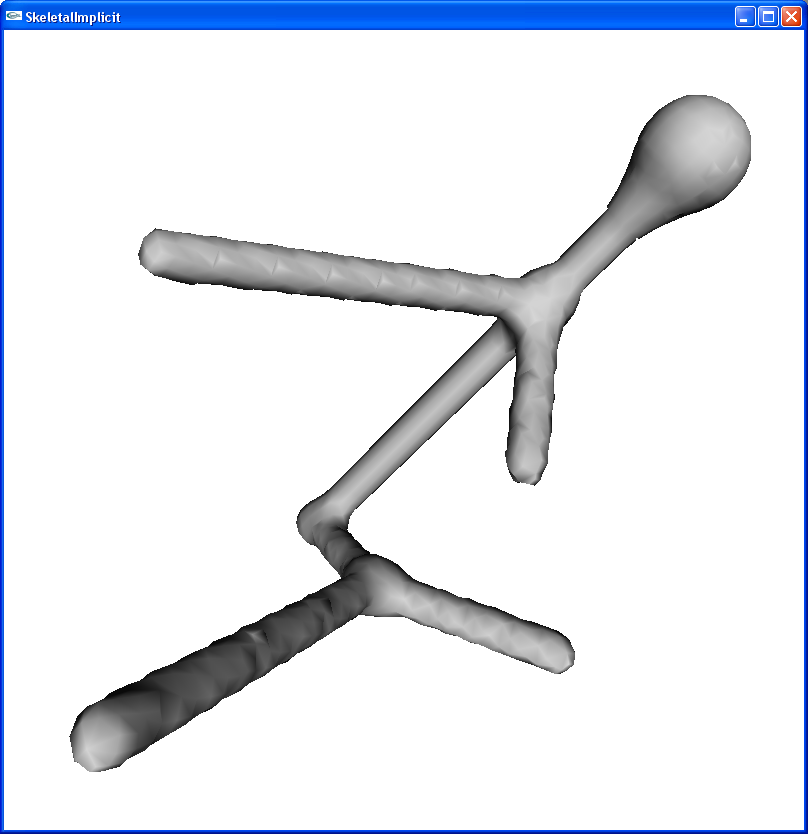
\includegraphics[width=0.3\textwidth]{../pictures/dynamicSkeletonPolygonized.png}}
  \caption{Skeleton to surface}
  \label{fig:animals}
\end{figure}

\subsection{By-products}

\begin{figure}[!h!]
  \centering
  \subfloat[Textured with a 3D noise function]{\label{bound}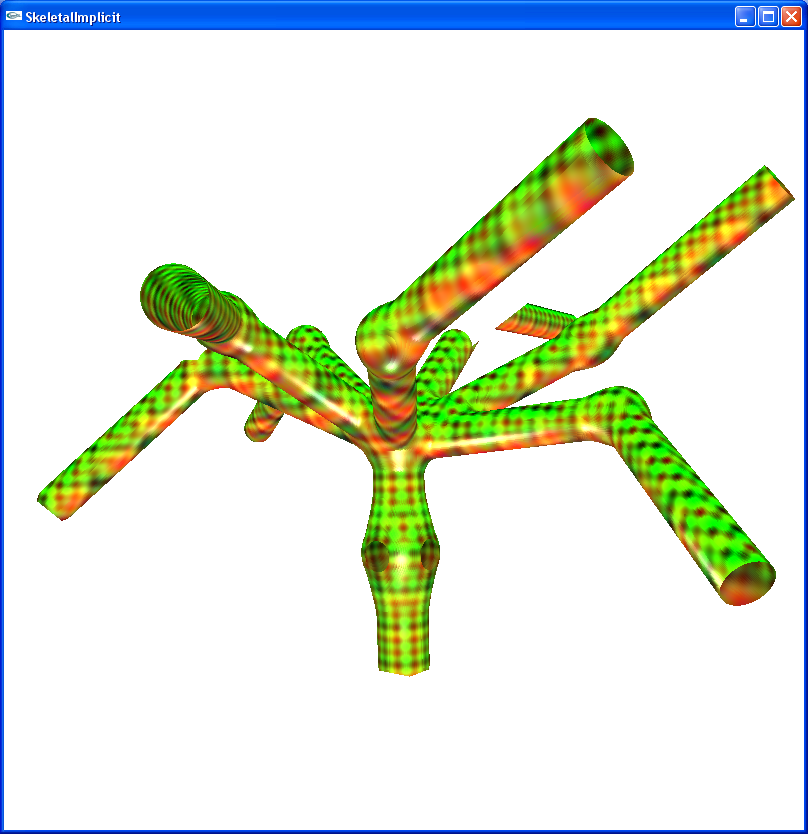
\includegraphics[width=0.5\textwidth]{../pictures/tree.png}}                
  \subfloat[Rendered in a voxel style]{\label{fig:tiger}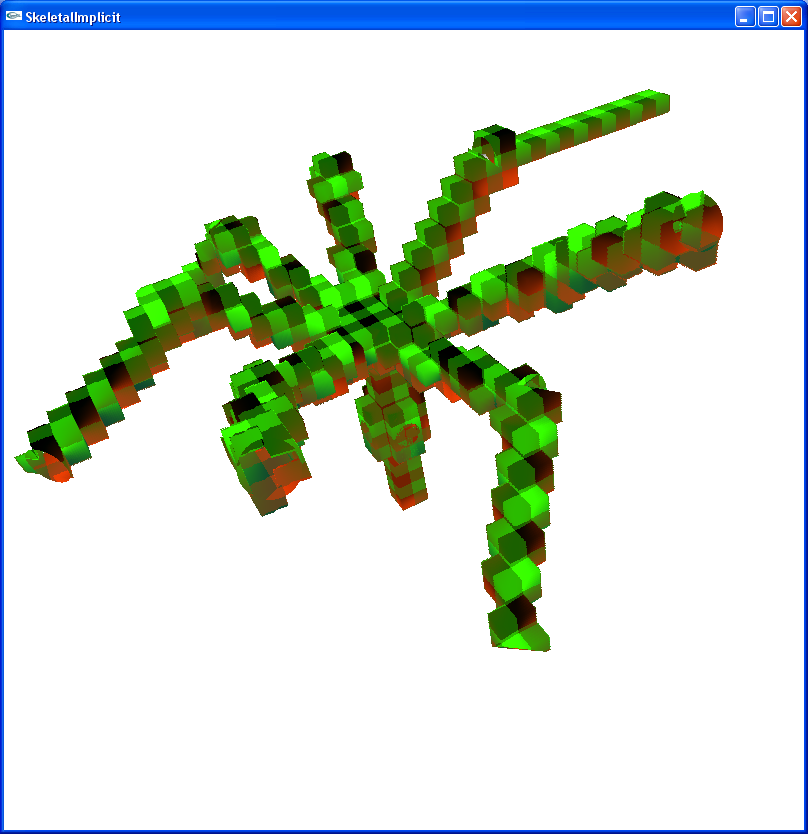
\includegraphics[width=0.5\textwidth]{../pictures/treeVoxelStyle2.png}}

  \caption{Other skeleton with effects}
  \label{fig:animals}
\end{figure}

\subsection{Remarks}

\begin{itemize}

\item{} Blending is good but too much blending is bad. forearm blends with upper arm but not with left foot! It gives me the idea that when ray marching, only the primitives of adjascent bones should be evaluated.
\begin{figure}[!h!]
\centering
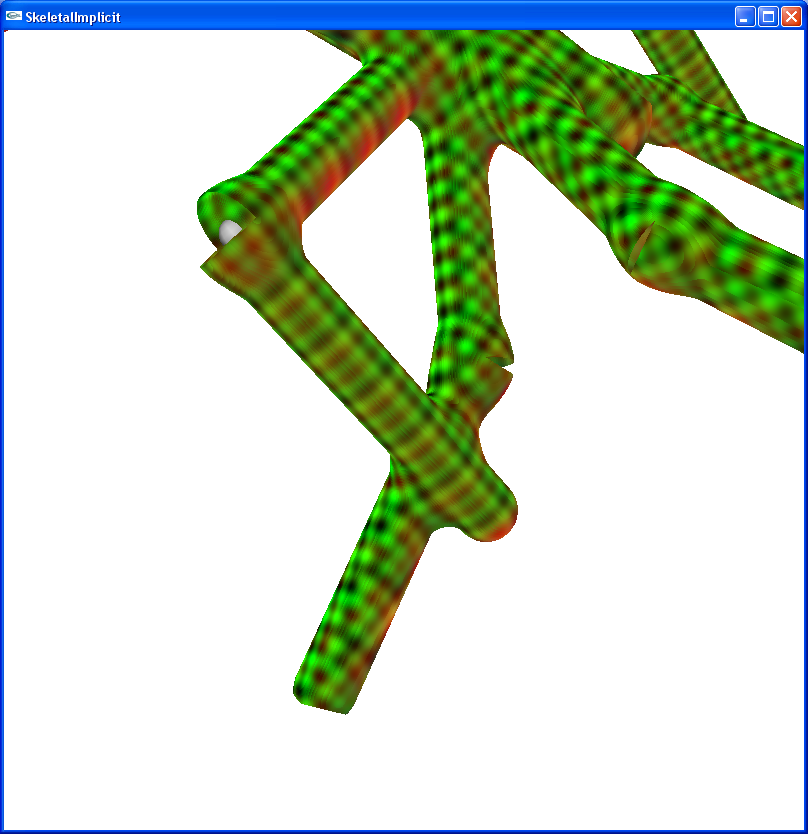
\includegraphics[scale=0.3]{../pictures/wrongblend.png}
\caption{wrong blending}
\label{bilb}
\end{figure}

\end{itemize}


\Section[simple]{Optimizing the ray tracing - Reading Notes}

\subsection{Goal}

Design an algorithm to raytrace efficiently a implicit surface defined by a skeleton.
\begin{itemize}

\item{} The algorithm must raytrace the surface efficiently, if possible as fast as rasterizing a mesh.
\item The algorithm must get the entire surface.
\item The algorithm must allow dynamic skeleton.
\item The algorithm must allow as many effect as possible.

\end{itemize}

How to speed up the ray-tracing?

\begin{itemize}

\item{} Shoot ray only where there is a surface intersection. Involves spatial subdivision techniques such as BVH, Octree, ... Or as we did send bounding primitives to the pipeline.
\item Speed up intersection. Choice of root finding algo, using geometry.
\item Evaluate only the primitives that contributes at the point of evaluation. spatial sorting.

\end{itemize}

\Section[simple]{Techniques for root finding}

Hart gives a good intro to different techniques in Ray-Tracing implicit surfaces.

\subsection{Polynomial Root Solving}

Works for algebraic surfaces (in our scope).

First work seems to be from Hanrahan \cite{Hanrahan:1983:RTA:800059.801136}. His method used "a symbolic
algebra system to automatically derive the
equation of intersection between the ray
and the surface and then solves this equation
using an exact polynomial root finding
algorithm". This implies converting the space function of the surface to a univariate function along the ray and then solve this polynomial equation.
Having the coefficients of the ray polynomial, numerical methods for root finding are used.

The same approach is used in \cite{Loop:2006:RGR:1179352.1141939} but the univariate ray polynomial is computed using Bezier tetrahedra.

\subsection{Interval analysis}

A common method to find root of a function along ray is to use interval analysis, isolating the root in an interval then refining this interval to approximate the root. \cite{Mitchell:1990:RRI:93267.93276}.

\subsection{Lipschitz methods}

Interval analysis can be improved by using the local Lipschitz constant of the function at each iteration.

\subsection{Sphere Tracing}

Another method to raytrace an implicit surface is to use sphere tracing \cite{springerlink:10.1007/s003710050084}. 
This method does not involve root finding but finds the first intersection of the ray with the surface.
This relies on knowing the distance of the current point on the ray to the surface. If this distance is less than $\epsilon$, we found the intersection, otherwise we know that we can move forward with the distance to the surface. It seems that in the case of convolution surfaces, we know this distance.

\Section[simple]{Acceleration data structure}

To address the problems of shooting rays only where the surface is and to evaluate only the primitives that contributes when marching the ray, we require a spatial data structure.

With metaballs or tubes (convolution surfaces) and with a distribution of compact support, we know that the primitives are zero outside a bounding volume (a sphere for a point primitive and a capsule for a tube).

One idea is to maintain on the GPU a bounding volume hierarchy as done \cite{Gourmel-2010-FBVH}.
This structure is used to limit the number of shooted rays and to decide which primitives have an effect.

\clearpage
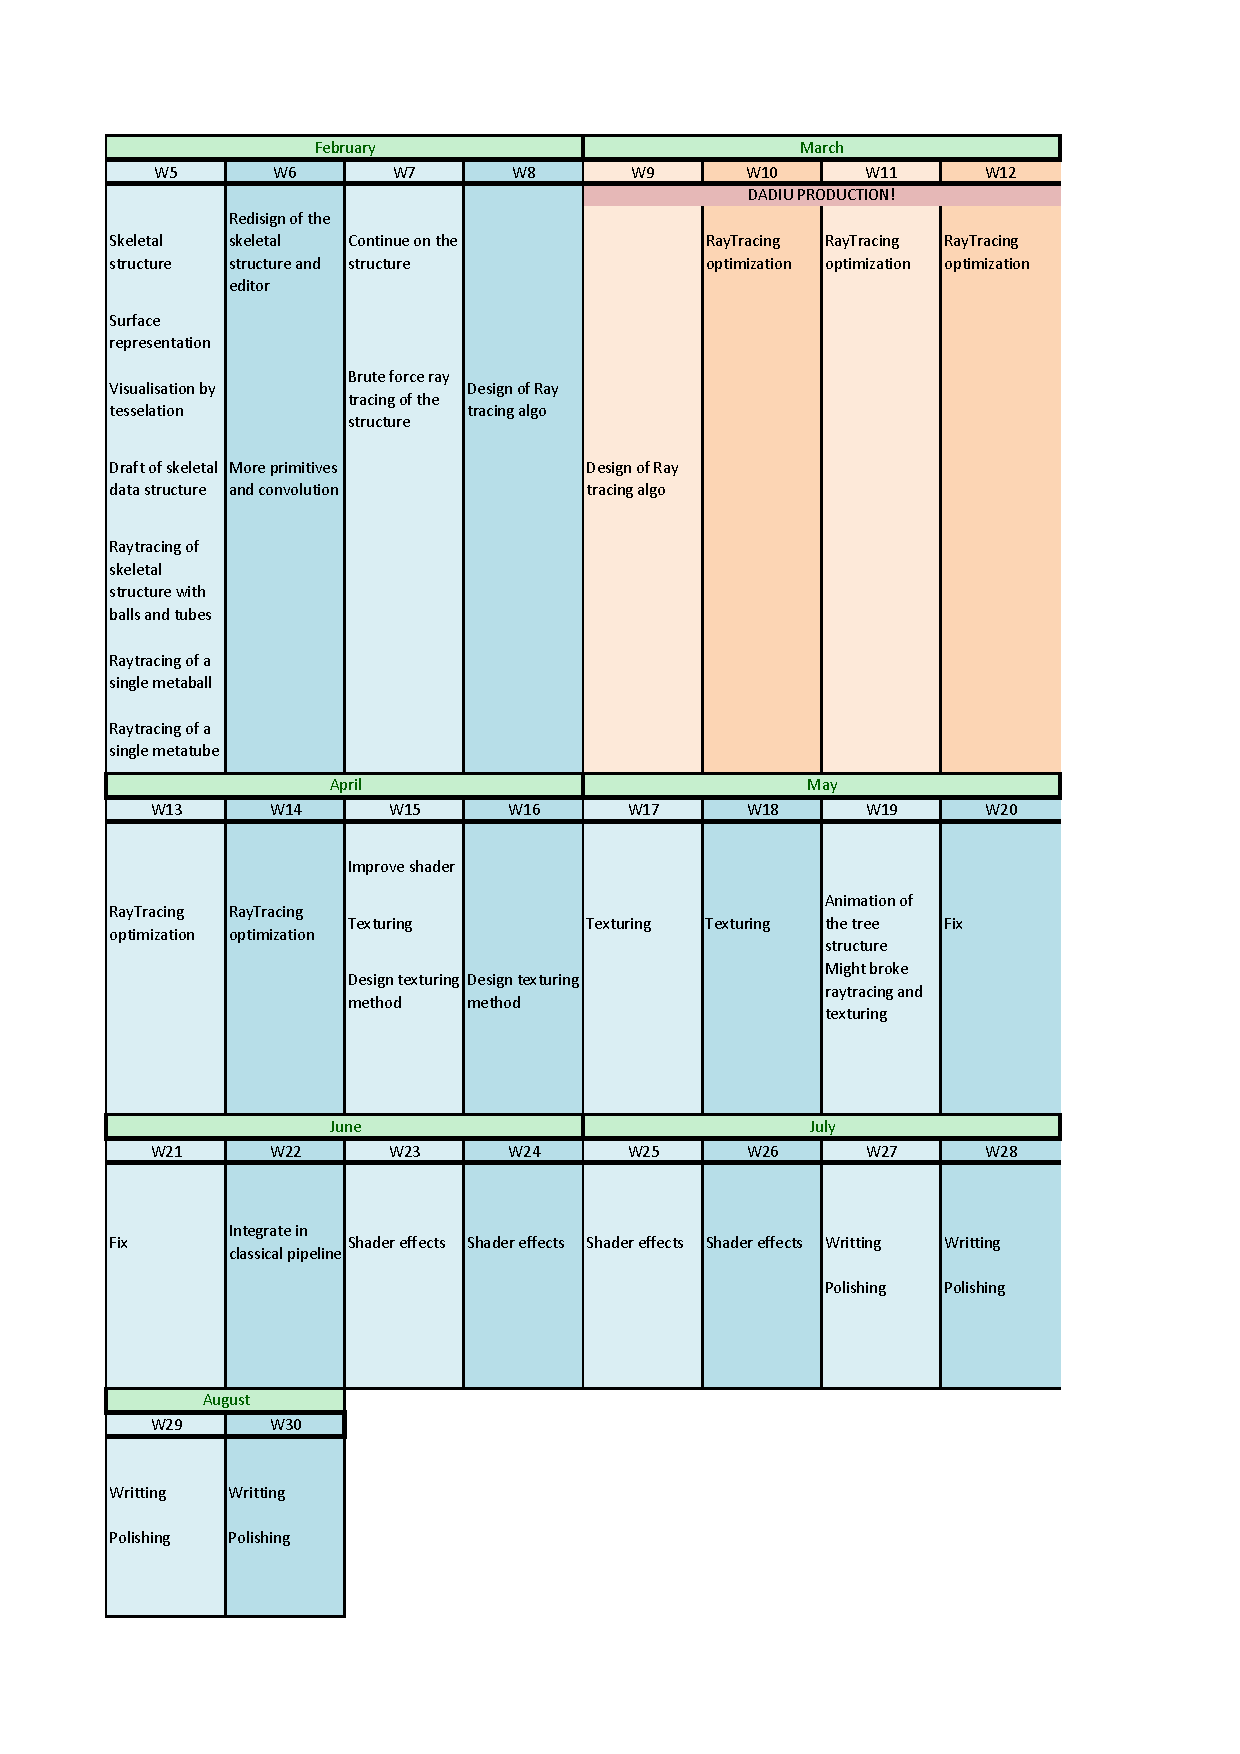
\includepdf{../../../projectPlan07-02.pdf} 

\bibliography{../../references} 
\bibliographystyle{alpha}

\end{document}
